%
%
%   AMASYA UNIVERSITESI
%   FEN BILIMLERI ENSTITUSU
%
%   LATEX TEZ SABLONU
%
%
%   Hazirlayan: Suleyman OGREKCI
%
%





%%%%%%%%%%%%%%%%%%%%%%%%%%%%%%%%%%%%%%
%%%%%
%%%%%   Bu dosya yazar tarafindan duzenlenmeli
%%%%%
%%%%%   Yorumlar dikkatlice okunmali
%%%%%
%%%%%%%%%%%%%%%%%%%%%%%%%%%%%%%%%%%%%%





%%%%%%%%%%%%%%%%%%%%%%%%%%%%%%%%%%%%%%
%%%%%
%%%%%   Icindekiler gibi listelerin hazirlanmasi icin
%%%%%
%%%%%   bu dosya iki (2) defa derlenmeli
%%%%%
%%%%%%%%%%%%%%%%%%%%%%%%%%%%%%%%%%%%%%










%%%%%%%%%%%%%%%%%%%%%%%%%%%%%%%%%%%%%%
%%%%%   Dokuman sinifi secimi
%%%%%%%%%%%%%%%%%%%%%%%%%%%%%%%%%%%%%%

\documentclass[
oneside, %Onlu arkali yazilacak ise bu satir silinecek
doktora, %Bu tez bir yuksek lisans tezi ise bu satir silinecek
]{aufbetez} %Bu satir degistirilmeyecek

%Bunlarin disinda ihtiyac duyuluyorsa diger book sinifi 
%opsiyonlari kullanilabilir

%%%%%%%%%%%%%%%%%%%%%%%%%%%%%%%%%%%%%%
%%%%%%%%%%%%%%%%%%%%%%%%%%%%%%%%%%%%%%




%%%%%%%%%%%%%%%%%%%%%%%%%%%%%%%%%%%%%%
%%%%%   kullanacaginiz paketleri ve makrolari
%%%%%   burada tanimlayabilirsiniz
%%%%%%%%%%%%%%%%%%%%%%%%%%%%%%%%%%%%%%

%%%%% tez yazim kilavuzuna aykiri paketler 
%%%%% (yazi tipini degistiren paketler gibi) kullanilmamali



\usepackage[utf8]{inputenc}
\usepackage{lipsum}
\usepackage{amsmath}
\usepackage{amssymb}



%Paket ve makro tanimlamalari burada bitsin

%%%%%%%%%%%%%%%%%%%%%%%%%%%%%%%%%%%%%%
%%%%%%%%%%%%%%%%%%%%%%%%%%%%%%%%%%%%%%






%%%%%%%%%%%%%%%%%%%%%%%%%%%%%%%%%%%%%%
%%%%%   Tez ve Yazar Bilgileri
%%%%%%%%%%%%%%%%%%%%%%%%%%%%%%%%%%%%%%

%%%%% Tez ve yazar bilgileri asagida girilmeli

\tezbasligi{AMASYA ÜNİVERSİTESİ LATEX TEZ ŞABLONU}%Tez basligi turkce
\thesistitle{AMASYA UNIVERSITY LATEX THESIS TEMPLATE}%Ingilizce baslik
\yazar{Süleyman ÖĞREKÇİ}%Tez yazari
\danisman{Prof. Dr. Adil MISIR}%Danisman unvani adi soyadi
\danismanuni{Amasya Üniversitesi}%Danisman universite
\danismanabd{Matematik}%Danisman anabilim dali
\ikincidanisman{Prof. Dr. RAMAZAN YILMAZ}%Ikinci danisman, yoksa bu satiri silin
\tezteslimtarihi{21}{06}{2021}%Tez teslim tarihi: {gun}{ay}{yil}
\sayfasayisi{92}%Tezin toplam sayfa sayisi
\ithafcumlesi{Bu çalışmayı Prof. Dr. Mehmet Demir'e ithaf ediyorum.}%Ithaf yoksa silin

%%%%%%%%%%%%%%%%%%%%%%%%%%%%%%%%%%%%%%
%%%%%%%%%%%%%%%%%%%%%%%%%%%%%%%%%%%%%%





%%%%%%%%%%%%%%%%%%%%%%%%%%%%%%%%%%%%%%
%%%%%   Savunma Bilgileri
%%%%%%%%%%%%%%%%%%%%%%%%%%%%%%%%%%%%%%

\enstitumuduru{Doç. Dr. Ümit YILDIRIM}%Enst. muduru unvan ad soyad
\tezsavunmatarihi{10}{10}{2021}%savunma tarihi: {gun}{ay}{yil}

%%%%% Savunma jurisi bilgileri asagida girilmeli
%%%%% Juri = Danisman + Baskan + Diger Uyeler

%Ilk juri uyesi danismandir

\juribaskani{Prof. Dr. Ahmet Ali YILMAZ}%Ikinci juri uyesi, juri baskani
\juribaskaniabd{Matematik}
\juribaskaniuni{Ankara Üniversitesi}

\juriuyebir{Doç. Dr. Mahmut DURAN}%Diger juri uyesi. Uc uye varsa bu sonuncusu olacak.
\juriuyebirabd{Matematik Eğitimi}
\juriuyebiruni{Gazi Üniversitesi}

%%%%% 5 veya 7 uyeli juri icin asagidaki gibi devam edilmeli

%\juriuyeiki{Doç. Dr. Musa KARA}%Uc uyeli juride bu yok
%\juriuyeikiabd{Makine Mühendisliği}
%\juriuyeikiuni{İstanbul Üniversitesi}
%
%\juriuyeuc{Dr. Öğr. Üy. Kerami BORAN}%Uc uyeli juride bu yok
%\juriuyeucabd{Matematik Eğitimi}
%\juriuyeucuni{Kastamonu Üniversitesi}
%
%\juriuyedort{Doç. Dr. Metin AK}%Uc veya bes uyeli juride bu yok
%\juriuyedortabd{Fizik}
%\juriuyedortuni{Amasya Üniversitesi}
%
%\juriuyebes{Doç. Dr. Feridun SARI}%Uc veya bes uyeli juride bu yok
%\juriuyebesabd{Matematik}
%\juriuyebesuni{Amasya Üniversitesi}

%%%%%%%%%%%%%%%%%%%%%%%%%%%%%%%%%%%%%%
%%%%%%%%%%%%%%%%%%%%%%%%%%%%%%%%%%%%%%







%%%%%%%%%%%%%%%%%%%%%%%%%%%%%%%%%%%
%%%%%
%%%%%   Belge baslatiliyor
%%%%%
%%%%%   OZEL SAYFALAR
%%%%%
%%%%%%%%%%%%%%%%%%%%%%%%%%%%%%%%%%%





\begin{document}
\shorthandoff{=}%Bu satiri silmeyin


\frontmatter%Bu satiri silmeyin




%%%%%%%%%%%%%%%%%%%%%%%%%%%%%%%%%%%%%%
%%%%%   Ic Kapak ve Bazi Ozel Sayfalar
%%%%%%%%%%%%%%%%%%%%%%%%%%%%%%%%%%%%%%

%%%%% Asagidaki uc satir silinmemeli

\ickapak%ic kapak sayfasini yazdirir
\tezkabulonaysayfasi%tez kabul onay sayfasini yazdirir
\ithafsayfasi%ithaf cumlesi verilmisse ithaf sayafisini yazdirir

%%%%%%%%%%%%%%%%%%%%%%%%%%%%%%%%%%%%%%
%%%%%%%%%%%%%%%%%%%%%%%%%%%%%%%%%%%%%%




%%%%%%%%%%%%%%%%%%%%%%%%%%%%%%%%%%%%%%
%%%%%   Etik Beyan
%%%%%%%%%%%%%%%%%%%%%%%%%%%%%%%%%%%%%%

%%%%% Etik beyan metnini duzenleyin

\begin{etikbeyan}
	Amasya Üniversitesi Fen Bilimleri Enstitüsü Tez Yazım Kurallarına uygun olarak hazırladığım bu tez çalışmasında;
	\begin{itemize}
		\item Tez içinde sunduğum verileri, bilgileri ve dokümanları akademik ve etik kurallar çer\-çe\-ve\-sin\-de elde ettiğimi,
		\item Tüm bilgi, belge, değerlendirme ve sonuçları bilimsel etik ve ahlak kurallarına uygun olarak sunduğumu,
		\item Tez çalışmasında yararlandığım eserlerin tümüne uygun atıfta bulunarak kaynak gös\-ter\-diği\-mi,
		\item Kullanılan verilerde herhangi bir değişiklik yapmadığımı,
		\item Bu tezde sunduğum çalışmanın özgün olduğunu
	\end{itemize}
	bildirir, aksi bir durumda aleyhime doğabilecek tüm hak kayıplarını kabullendiğimi beyan ederim.
\end{etikbeyan}

%%%%%%%%%%%%%%%%%%%%%%%%%%%%%%%%%%%%%%
%%%%%%%%%%%%%%%%%%%%%%%%%%%%%%%%%%%%%%





%%%%%%%%%%%%%%%%%%%%%%%%%%%%%%%%%%%%%%
%%%%%   Ozet
%%%%%%%%%%%%%%%%%%%%%%%%%%%%%%%%%%%%%%

%%%%% Ozet metnini duzenleyin

\begin{ozet}
	\lipsum[1-2]
	\anahtarkelimeler{anahtar, kelime, deneme, şablon}
\end{ozet}

%%%%%%%%%%%%%%%%%%%%%%%%%%%%%%%%%%%%%%
%%%%%%%%%%%%%%%%%%%%%%%%%%%%%%%%%%%%%%





%%%%%%%%%%%%%%%%%%%%%%%%%%%%%%%%%%%%%%
%%%%%   Abstract
%%%%%%%%%%%%%%%%%%%%%%%%%%%%%%%%%%%%%%

%%%%% Abstract (ingilizce ozet) metnini duzenleyin

\begin{abstract}
	\lipsum[5]
	\keywords{key, word, trial, template}
\end{abstract}

%%%%%%%%%%%%%%%%%%%%%%%%%%%%%%%%%%%%%%
%%%%%%%%%%%%%%%%%%%%%%%%%%%%%%%%%%%%%%





%%%%%%%%%%%%%%%%%%%%%%%%%%%%%%%%%%%%%%
%%%%%   On Soz
%%%%%%%%%%%%%%%%%%%%%%%%%%%%%%%%%%%%%%

%%%%% On soz ve tesekkur metnini duzenleyin

\begin{onsoz}
	\lipsum[1-3]
\end{onsoz}

%%%%%%%%%%%%%%%%%%%%%%%%%%%%%%%%%%%%%%
%%%%%%%%%%%%%%%%%%%%%%%%%%%%%%%%%%%%%%





%%%%%%%%%%%%%%%%%%%%%%%%%%%%%%%%%%%%%%
%%%%%   Icindekiler ve Diger Dizinler
%%%%%%%%%%%%%%%%%%%%%%%%%%%%%%%%%%%%%%

%%%%% Diger dizinlerin icerigi bos ise yazdirilmaz.
%%%%% Asagidaki bes satiri silmeyin.

\icindekiler
\cizelgelerdizini
\sekillerdizini
\resimlerlerdizini
\haritalardizini

%%%%%%%%%%%%%%%%%%%%%%%%%%%%%%%%%%%%%%
%%%%%%%%%%%%%%%%%%%%%%%%%%%%%%%%%%%%%%





%%%%%%%%%%%%%%%%%%%%%%%%%%%%%%%%%%%%%%
%%%%%   Simgeler ve Kisaltmalar Dizini
%%%%%%%%%%%%%%%%%%%%%%%%%%%%%%%%%%%%%%

%%%%% Simgeler ve kisaltmalar dizinini duzenleyin
%%%%% Tezinizde bu dizin yoksa bunlari silin.

\begin{simgelerdizini}
	\begin{table}[htbp]
		\doublespacing
			\begin{tabular}{l@{\hskip 4.5cm}l}
				\textbf{Simgeler} & \textbf{Açıklama}                \\
				$\mathbb{R}$        & Reel Sayılar Kümesi     \\
				$\mathbb{C}$        & Kompleks Sayılar Kümesi \\
				e        & Euler Sabiti            \\
				$\Gamma$    & Gama Fonksiyonu        \\
				&\\
				\textbf{Kısaltmalar} & \textbf{Açıklama}                \\
				TMD        & Türk Matematik Derneği     \\
				TDK        & Türk Dil Kurumu \\
				IR        & Kırmızı-altı            \\
				CFT    & Kalkülüsün Temel Teoremi        
			\end{tabular}%
	\end{table}
\end{simgelerdizini}

%%%%%%%%%%%%%%%%%%%%%%%%%%%%%%%%%%%%%%
%%%%%%%%%%%%%%%%%%%%%%%%%%%%%%%%%%%%%%





%%%%%%%%%%%%%%%%%%%%%%%%%%%%%%%%%%%
%%%%%
%%%%%   OZEL SAYFALAR BITTI
%%%%%
%%%%%%%%%%%%%%%%%%%%%%%%%%%%%%%%%%%






\mainmatter% Bunu silmeyin






%%%%%%%%%%%%%%%%%%%%%%%%%%%%%%%%%%%%%%
%%%%%%%%%%%%%%%%%%%%%%%%%%%%%%%%%%%%%%
%%%%%%%%%%%%%%%%%%%%%%%%%%%%%%%%%%%%%%
%%%%%
%%%%%   TEZ GOVDESI  BURADA BASLIYOR
%%%%%
%%%%%%%%%%%%%%%%%%%%%%%%%%%%%%%%%%%%%%
%%%%%%%%%%%%%%%%%%%%%%%%%%%%%%%%%%%%%%
%%%%%%%%%%%%%%%%%%%%%%%%%%%%%%%%%%%%%%





\chapter{GİRİŞ}
\lipsum[1] $x^2+\lim\limits_{t\to\infty}f(t)-\sum_{k=1}^{n}\frac{1-k}{k!}$ ve\footnote{bu bir dipnottur, deneme amaçlı yazılmıştır. Gerektiği yerde metne dipnotlar eklenebilir.} $$\int_{a}^{b}f(x)\cos(xt)dx$$
\begin{itemize}
	\item madde bir, bu bir deneme metnidir
	\item madde iki, bu bir deneme metnidir
	\item madde üç, bu bir deneme metnidir
	\item madde dört, bu bir deneme metnidir
\end{itemize}


\begin{definition}
	\label{tanim-1}
	Bu bir tanımdır.
\end{definition}

\begin{theorem}
	\label{teorem-1}
	Bu bir teorem ifadesidir, aşağıda bunun ispatı da yer alacak.
\end{theorem}

\begin{proof}
	Bu metin, Teorem \ref{teorem-1}'in ispatını içerir, metin içinde \cite{ogrekci18} şeklinde atıf verilebilir.
\end{proof}

\begin{corollary}
	\label{sonuc-1}
	Bu bir sonuç metnidir.
\end{corollary}

\begin{lemma}
	\label{lemma-1}
	Bu da bir yardımcı teorem metnidir. Teorem \ref{teorem-1} için olduğu gibi bunun da ispatı aşağıda yer alacak.
\end{lemma}

\begin{proof}
	Bu metin, Yardımcı Teorem \ref{lemma-1}'in ispatıdır.
\end{proof}


\begin{example}
	\label{ornek-1}
	Bu bir örnek metnidir.
\end{example}

\begin{remark}
	\label{uyari-1}
	bu bir uyarı metnidir.
\end{remark}

\section{Birinci Alt Bölüm}
\lipsum

\begin{table}[htbp]
\begin{center}
		\begin{tabular}{|c|c|}
	\hline 
	1 & 2 \\ 
	\hline 
	3 & 4 \\ 
	\hline 
\end{tabular}
\end{center}
\caption{bir tablo\label{tablo-1}}
\end{table}

Tablo \ref{tablo-1} gereği \lipsum[2]

\begin{figure}[htbp]
	\centering
	
\includegraphics[scale=3.5]{logo}
	\caption{Bu bir şekildir.}
	\label{sekil-1}
\end{figure}


\subsection{Bir alt alt bölüm}
\lipsum

\subsection{Başka bir alt alt bölüm}
\lipsum

\section{İkinci Alt Bölüm}
\lipsum
\begin{table}[htbp]
	\begin{center}
		\begin{tabular}{|c|c|}
			\hline 
			5 & 6 \\ 
			\hline 
			7 & 8 \\ 
			\hline 
		\end{tabular}
	\end{center}
	\caption{bir tablo\label{tablo-2}}
\end{table}
\section{Üçüncü Alt Bölüm}
\lipsum

\begin{figure}[htbp]
	\centering
	
\includegraphics[scale=4.5]{logo}
	\caption{Bu başka bir şekildir.}
	\label{sekil-2}
\end{figure}

\begin{thesispicture}{Bir resim denemesi}
	\begin{center}
		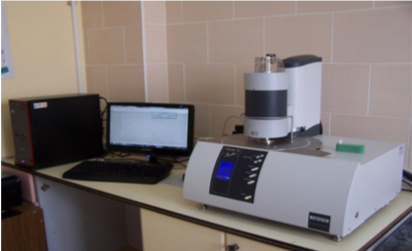
\includegraphics[scale=0.75]{resim}
	\end{center}
\end{thesispicture}
\lipsum[1-3]

\chapter{KURAMSAL ÇERÇEVE}
\lipsum

\section{Bir Alt Bölüm}
\lipsum

\section{Bir Alt Bölüm}
\lipsum

\subsection{Bir alt alt bölüm}
\lipsum

\subsection{Bir alt alt bölüm}
\lipsum

\section{Bir Alt Bölüm}
\lipsum

\chapter{LİTERATÜR İNCELEMESİ}
\lipsum

\section{Bir Alt Bölüm}
\lipsum

\subsection{Bir alt alt bölüm}
\lipsum

\subsection{Bir alt alt bölüm}
\lipsum

\section{Bir Alt Bölüm}
\lipsum

\section{Bir Alt Bölüm}
\lipsum

\subsection{Bir alt alt bölüm}
\lipsum

\subsection{Bir alt alt bölüm}
\lipsum

\chapter{TEMEL TEOREMLER}
\lipsum
\begin{table}[htbp]
	\begin{center}
		\begin{tabular}{|c|c|}
			\hline 
			9 & 10 \\ 
			\hline 
			11 & 12 \\ 
			\hline 
		\end{tabular}
	\end{center}
	\caption{bir tablo\label{tablo-3}}
\end{table}

\section{Bir Alt Bölüm}
\lipsum

\subsection{Bir alt alt bölüm}
\lipsum

\subsection{Bir alt alt bölüm}
\lipsum

\section{Bir Alt Bölüm}
\lipsum

\subsection{Bir alt alt bölüm}
\lipsum

\subsection{Bir alt alt bölüm}
\lipsum

\chapter{SONUÇ VE ÖNERİLER}
\lipsum


\begin{thesispicture}{Bir resim denemesi}
		\begin{center}
		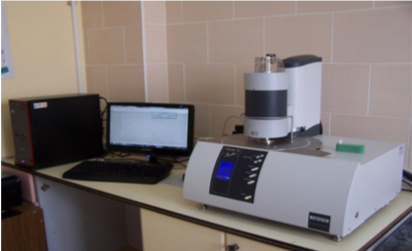
\includegraphics[scale=0.75]{resim}
	\end{center}
\end{thesispicture}

\lipsum

\begin{thesispicture}{Bir resim denemesi}
		\begin{center}
		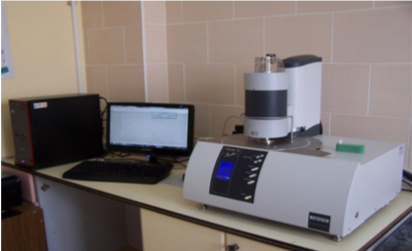
\includegraphics[scale=0.75]{resim}
	\end{center}
\end{thesispicture}

\lipsum

\begin{thesismap}{Bir harita denemesi}
	\begin{center}
		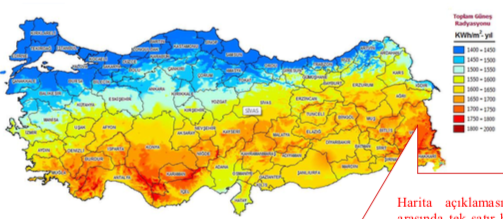
\includegraphics[scale=0.75]{harita}
	\end{center}
\end{thesismap}

\lipsum

\begin{thesismap}{Bir harita denemesi}
	\begin{center}
		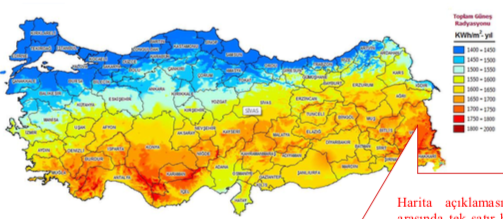
\includegraphics[scale=0.75]{harita}
	\end{center}
\end{thesismap}

Bu çalışmada \cite{lamport94} eseri \lipsum[2]

 ayrıca \cite[s.~123]{lamport94} incelenirse \lipsum[50]







%%%%%%%%%%%%%%%%%%%%%%%%%%%%%%%%%%%%%%
%%%%%
%%%%%   TEZ GOVDESI  BURADA BITIYOR
%%%%%
%%%%%%%%%%%%%%%%%%%%%%%%%%%%%%%%%%%%%%






\backmatter%bunu silmeyin





%%%%%%%%%%%%%%%%%%%%%%%%%%%%%%%%%%%%%%
%%%%%
%%%%%   KAYNAKLAR, EKLER, OZGECMİS
%%%%%
%%%%%%%%%%%%%%%%%%%%%%%%%%%%%%%%%%%%%%





%%%%%%%%%%%%%%%%%%%%%%%%%%%%%%%%%%%%%%
%%%%%   Kaynaklar
%%%%%%%%%%%%%%%%%%%%%%%%%%%%%%%%%%%%%%


%%%%% Kaynakca basliyor

%%%%% Asagidaki iki satir degistirilmemeli, silinmemeli
\renewcommand\bibname{\centerline{KAYNAKLAR}\global\def\bibname{KAYNAKLAR}}
\addcontentsline{toc}{chapter}{KAYNAKLAR}


%%%%%%%%%%%%%%%%%%%%%%%%%%%%%%%%%%%%%%
%%%%%
%%%%%   Kaynakca icerigi asagida duzenlenmeli
%%%%%
%%%%%   Temsili olarak yazilmistir
%%%%%
%%%%%   Tez yazim kilavuzundaki kurallara
%%%%%
%%%%%   göre duzenlenmelidir
%%%%%
%%%%%%%%%%%%%%%%%%%%%%%%%%%%%%%%%%%%%%

\begin{thebibliography}{99}
	
	\bibitem{lamport94}
	Leslie Lamport,
	\textit{\LaTeX: a document preparation system},
	Addison Wesley, Massachusetts,
	2nd edition,
	1994.
	
	\bibitem{ogrekci18}
	Süleyman Öğrekçi (2018),
	\textit{Temel Matematik Analiz},
	Nobel Akademik Yayıncılık, Ankara,
	2018.
	
\end{thebibliography}

%%%%%%%%%%%%%%%%%%%%%%%%%%%%%%%%%%%%%%
%%%%%%%%%%%%%%%%%%%%%%%%%%%%%%%%%%%%%%






%%%%%%%%%%%%%%%%%%%%%%%%%%%%%%%%%%%%%%
%%%%%   Ekler
%%%%%%%%%%%%%%%%%%%%%%%%%%%%%%%%%%%%%%


%%%%% Ekler icin kapak
%%%%% Ihtıyac yoksa silinmeli
\eklerkapagi


%%%%% Ekler Basliyor
%%%%% Ihtiyac kadar asagidakiler tekrarlanabilir

\textbf{Ek-1: Bir Ek Ögesi}%Ek basligi
\addcontentsline{toc}{chapter}{Ek-1: Bir Deneme Ek Ögesi}%Ek bilgisini icindekilere kaydet

\lipsum[1-3]%Ek icerigi

\clearpage%Yeni ek icin yeni sayfaya atla

\textbf{Ek-2: Başka Bir Ek}
\addcontentsline{toc}{chapter}{Ek-2: Başka Bir Ek}

\lipsum[1-3]


\clearpage%Yeni ek icin yeni sayfaya atla

\textbf{Ek-3: Başka Bir Ek}
\addcontentsline{toc}{chapter}{Ek-3: Başka Bir Ek}

\lipsum[1-3]

%%%%%%%%%%%%%%%%%%%%%%%%%%%%%%%%%%%%%%
%%%%%%%%%%%%%%%%%%%%%%%%%%%%%%%%%%%%%%






%%%%%%%%%%%%%%%%%%%%%%%%%%%%%%%%%%%%%%
%%%%%   Ozgecmis
%%%%%%%%%%%%%%%%%%%%%%%%%%%%%%%%%%%%%%

%%%%% Ozgecmisinizi duzenleyin

\begin{ozgecmis}
	\begin{table}[htbp]
		\doublespacing
		\setlength{\tabcolsep}{18pt}
		\begin{tabular}{lll}
			\textbf{Kişisel Bilgiler}        &                         &                                 \\
			Adı-Soyadı              & : Süleyman Öğrekçi      & \multirow{5}{*}{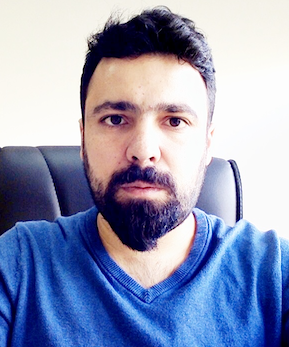
\includegraphics[scale=0.35]{profilresmi}}   \\
			Uyruğu                  & : Türkiye Cumhuriyeti   &                                 \\
			Doğum tarihi ve yeri    & : 01/01/1935 Manavgat   &                                 \\
			Medeni hali             & : Evli                  &                                 \\
			e-posta                 & : s.ogrekci@gmail.com   &                                 \\
			\textbf{Eğitim Derecesi}         & \textbf{Okul/Program}            & \textbf{Mezuniyet Yılı}                  \\
			Lisans                  & Selçuk Üniversitesi     & 2001                            \\
			Yüksek Lisans           & Gazi Üniversitesi       & 2006                            \\
			\textbf{İş Deneyimi/Yıl}         & \textbf{Çalıştığı Yer}           & \textbf{Görevi}                          \\
			2007-                   & Amasya Üniversitesi     & Araştırma Görevlisi             \\
			\textbf{Yabancı Dil}             &                         &                                 \\
			İngilizce               &                         &                                 \\
			\multicolumn{3}{l}{\textbf{Bilimsel Faaliyetler (Yayınlar, Bildiriler, Katıldığı Projeler)}} \\
			\multicolumn{3}{l}{
				Yayınlar buraya yazılabilir..
			}
		\end{tabular}%
	\end{table}
\end{ozgecmis}

%%%%%%%%%%%%%%%%%%%%%%%%%%%%%%%%%%%%%%
%%%%%%%%%%%%%%%%%%%%%%%%%%%%%%%%%%%%%%






\end{document}